
\documentclass[12pt]{article}

%%%%%%%%%%%%%%%%%%%%%%%%%%%%%%%%%%%%%%%%%%%%%%%%%%%%%%%%%%%%%%%%%%%%%%%%%%%%%%%
% PACKAGE INCLUDING
%%%%%%%%%%%%%%%%%%%%%%%%%%%%%%%%%%%%%%%%%%%%%%%%%%%%%%%%%%%%%%%%%%%%%%%%%%%%%%%
\usepackage{amsmath}
\usepackage{graphicx}
\usepackage{hyperref}
\usepackage[utf8]{inputenc}
\usepackage[T5]{fontenc}
\usepackage{fancyhdr}
\usepackage{geometry}
\usepackage{amsfonts} 

\usepackage{csquotes}
\usepackage{listings}
\usepackage{enumitem}
\usepackage{subfiles}
\usepackage{tcolorbox}
\usepackage{colortbl}
\usepackage{float}
\usepackage{caption}
\usepackage{circuitikz}
\usepackage{tikz}
\usepackage{bm}
\usepackage{spverbatim}

%%%%%%%%%%%%%%%%%%%%%%%%%%%%%%%%%%%%%%%%%%%%%%%%%%%%%%%%%%%%%%%%%%%%%%%%%%%%%%%
% FORMATTING
%%%%%%%%%%%%%%%%%%%%%%%%%%%%%%%%%%%%%%%%%%%%%%%%%%%%%%%%%%%%%%%%%%%%%%%%%%%%%%%
\geometry{
    a4paper,
    total={170mm,250mm},
    left=20mm,
    top=30mm,
 }
\hypersetup{
    colorlinks=true,
    linkcolor=blue,
    filecolor=magenta,      
    urlcolor=blue,
    citecolor=blue
}

\pagestyle{fancy}
\fancyhf{}
\rhead{19120729}
\lhead{Bùi Ngọc Thảo Vy}
\rfoot{Trang \thepage}\setlength{\parindent}{0pt}
\setlength{\parskip}{0.3em}
\setlength{\headheight}{15pt}
\graphicspath{ {./images/} }

\setcounter{secnumdepth}{4}
\setcounter{tocdepth}{4}

\usetikzlibrary{matrix,calc}

%%%%%%%%%%%%%%%%%%%%%%%%%%%%%%%%%%%%%%%%%%%%%%%%%%%%%%%%%%%%%%%%%%%%%%%%%%%%%%%
% DEFINE NEW COMMAND
%%%%%%%%%%%%%%%%%%%%%%%%%%%%%%%%%%%%%%%%%%%%%%%%%%%%%%%%%%%%%%%%%%%%%%%%%%%%%%%
\newcommand{\SubItem}[1]{
    {\setlength\itemindent{15pt} \item[-] #1}
}

\newcommand\crule[3][black]{\textcolor{#1}{\rule{#2}{#3}}}


%%%%%%%%%%%%%%%%%%%%%%%%%%%%%%%%%%%%%%%%%%%%%%%%%%%%%%%%%%%%%%%%%%%%%%%%%%%%%%%
% DOCUMENT
%%%%%%%%%%%%%%%%%%%%%%%%%%%%%%%%%%%%%%%%%%%%%%%%%%%%%%%%%%%%%%%%%%%%%%%%%%%%%%%
\title{Kiểm tra kết thúc học phần môn Toán tổ hợp}

\author{LỚP 19CTT4}

\date{2021–07–05}


\begin{document}
\begin{sloppypar}

\begin{titlepage}
    
    \newcommand{\HRule}{\rule{\linewidth}{0.5mm}} % Defines a new command for the horizontal lines, change thickness here
    
    \center % Center everything on the page
    \vspace*{\fill}
     
    \textsc{\LARGE Đại học Khoa học Tự nhiên}\\[0.2cm]
    \textsc{\large Đại học Quốc gia TP. HCM }\\[1.5cm] 
    \textsc{\Large KHOA CÔNG NGHỆ THÔNG TIN}\\[0.2cm] 
    \textsc{\large LỚP 19CTT4 }\\[0.5cm]
    \HRule \\[0.4cm]
    { \huge \bfseries Kiểm tra kết thúc học phần môn\break 
    Thực hành Toán tổ hợp}\\[0.4cm] % Title of your document
    \HRule \\[1.5cm]
    \LARGE \textbf {Họ và tên: Bùi Ngọc Thảo Vy \\}
    \LARGE \textbf {MSSV: 19120729 \\}
    
    \begin{minipage}{1\textwidth}
    \begin{center}
        \LARGE Ngày 05/07/2021
    \end{center}
    \end{minipage}\\[2cm]
    \vspace*{\fill} % Fill the rest of the page with whitespace
    \end{titlepage}


    % MỤC LỤC
    \renewcommand*\contentsname{\begin{center} \LARGE Mục lục \end{center}}
    \tableofcontents
    \pagebreak
\section{Bài 1}
\subsection{Câu A: Lên cầu thang}

\begin{tcolorbox}
    \textbf{Đề bài:} Một cầu thang có \(n\) bậc, mỗi lần bước có thể bước lên 1 bậc hay 2 bậc. Có bao nhiêu cách đi hết cầu thang này? (đây chính là dãy Fibonaxi)
\end{tcolorbox}

- Gọi \(a_{n}\) là số cách bước lên cầu thang có \(n\) bậc. \\
- Do một lần có thể bước lên 1 hoặc 2 bậc nên ta có 2 cách để bước lên bậc thang thứ \(n\):

\begin{itemize}
    \item Từ bậc \(n - 1\)
    \item Từ bậc \(n - 2\)
\end{itemize}

- Với mỗi cách, ta lần lượt có \(a_{n-1}\) và \(a_{n - 2}\) cách. \\
\begin{center}
    {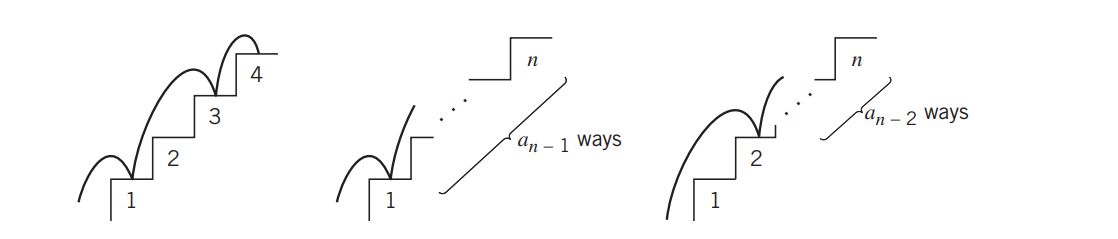
\includegraphics[width=16cm]{ex1a.png}}
\end{center}
- Theo nguyên lý cộng, ta có:

\begin{equation*}
    a_{n} = a_{n-1} + a_{n-2}
\end{equation*}

- Để bước lên bậc thang thứ 1, ta có 1 cách \(\Rightarrow a_{1} = 1\) \\
- Để bước lên bậc thang thứ 2, ta có 2 cách \(\Rightarrow a_{2} = 2\) \\
- Mà, ta lại có \(a_{2} = a_{0} + a_{1} \Leftrightarrow a_{0} = a_{2} - a_{1} = 2 - 1 = 1\). Từ đó suy ra:


    \[
    \begin{cases}
        a_{n} & = a_{n-1} + a_{n-2} \\             
        a_{0} & = a_{1} = 1; a_{2} = 2   
    \end{cases}
    \]

- Sử dụng Maple để giải hệ thức đệ quy, ta được:

\begin{verbatim}
    f := rsolve({a(0) = 1, a(1) = 1, a(n) = a(n-1) + a(n-2)}, a(n)): simplify(f)
\end{verbatim}

\begin{equation*}
    a_{n} = \left(\frac{1}{2} - \frac{\sqrt{5}}{10}\right)\left(\frac{-\sqrt{5}}{2} + \frac{1}{2}\right)^{n} + \left(\frac{1}{2} + \frac{\sqrt{5}}{10}\right)\left(\frac{\sqrt{5}}{2} + \frac{1}{2}\right)^{n}
\end{equation*}

\subsection{Câu B: Chia mặt phẳng}
\begin{tcolorbox}
    \textbf{Đề bài:} Tìm số miền tối đa có thể có khi chia mặt phẳng bởi \(n\) đường thẳng.
\end{tcolorbox}

\begin{center}
    {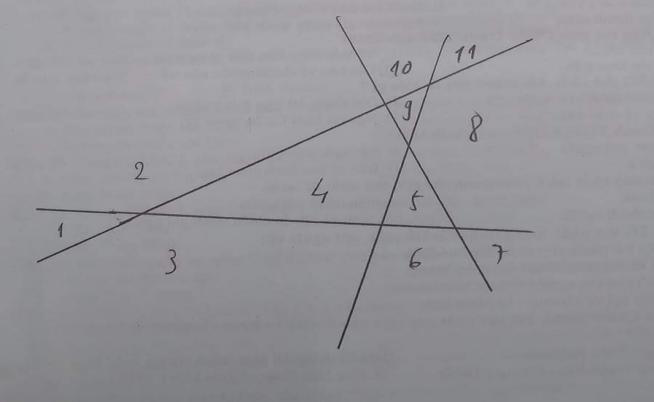
\includegraphics[width=8cm]{1b.png}}
\end{center}

- Gọi \(a_{n}\) là số mặt phẳng tối đa có thể có khi chia mặt phẳng bởi \(n\) đường thẳng. \\
- Đầu tiên, chúng ta khảo sát số miền tối đa có thể có đối với các giá trị \(n\) đường thẳng ban đầu như sau:

\begin{itemize}
    \item Với 0 đường đẳng (\(n = 0\)), ta thu được 1 mặt phẳng \(\Rightarrow a_{0} = 1\)
    \item Với 1 đường đẳng (\(n = 1\)), ta thu được 2 mặt phẳng \(\Rightarrow a_{1} = 2\)
    \item Với 2 đường thằng (\(n = 2\)), ta thu được 4 mặt phẳng \(\Rightarrow a_{2} = 4\)
    \item Với 3 đường thẳng (\(n = 3\)), ta thu được 7 mặt phẳng \(\Rightarrow a_{3} = 7\)
\end{itemize}

\begin{center}
    {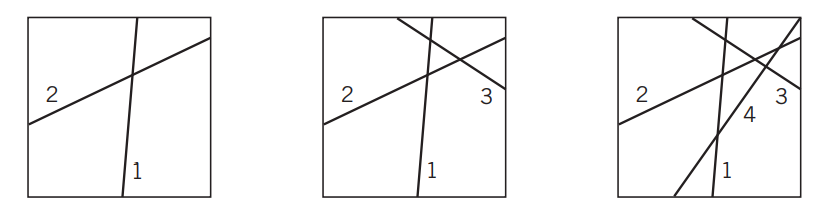
\includegraphics[width=16cm]{ex1b.png}}
\end{center}

- Như vậy, ta được dãy như sau:

\begin{equation*}
    a_{n} = a_{n - 1} + a_{n}
\end{equation*}

- Từ đó suy ra:

\[
    \begin{cases}
        a_{n} & = a_{n - 1} + n \\             
        a_{0} & = 1; a_{1} = 2   
    \end{cases}
    \]

- Sử dụng Maple để giải hệ thức đệ quy, ta được:

\begin{verbatim}
    f := rsolve({a(0) = 1, a(1) = 2, a(n) = a(n-1) + n}, a(n)): simplify(f)
\end{verbatim}

\begin{equation*}
    a_{n} = \frac{1}{2}n^{2} + \frac{1}{2}n + 1
\end{equation*}

\subsection{Câu C: Tháp Hà Nội}
\begin{tcolorbox}
    \textbf{Đề bài:} Có 3 cột 1,2 và 3. Có \(n\) đĩa nằm ở cột 1 được sắp xếp theo bán kính nhỏ dần từ dưới lên trên. Tìm số lần tối thiểu để chuyển tất cả n đĩa này sang cột khác sao cho thỏa mãn quy tắc:  đĩa có bán kính nhỏ hơn luôn nằm ở trên.
\end{tcolorbox}

\begin{center}
    {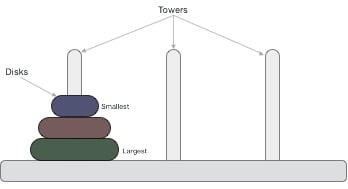
\includegraphics[width=8cm]{toh.png}}
\end{center}

- Gọi \(a_{n}\) là số lần tối thiểu để chuyển tất cả \(n\) đĩa này sang cột khác sao cho thỏa mãn quy tắc: đĩa có bán kính nhỏ hơn luôn nằm ở trên. \\
- Để chuyển \(n\) đĩa từ cột 1 sang cột 2:
\begin{itemize}
    \item Chuyển \(n\) đĩa từ cột 1 sang cột 3 \(\Rightarrow \text{Có } a_{n-1} \text{ cách.}\)
    \item Chuyển đĩa lớn nhất từ cột 1 sang cột 2 \(\Rightarrow \text{Có } 1 \text{ cách.}\)
    \item Chuyển các đĩa còn lại từ cột 3 về cột 1 \(\Rightarrow \text{Có } a_{n-1} \text{ cách.}\)
\end{itemize} 

- Theo nguyên lý cộng, ta có:

\begin{equation*}
    a_{n} = 2a_{n-1} + 1
\end{equation*}

- Từ đó suy ra:

\[
    \begin{cases}
        a_{n} & = 2a_{n - 1} + 1 \\             
        a_{1} & = 1 
    \end{cases}
    \]

%- Mặc khác, ta lại có trường hợp chuyển 1 đĩa như sau:

%\begin{align*}
%    a_{1} & = 1 \\
%    \Leftrightarrow a_{1} & = 2a_{0} + 1 \\
%    \Leftrightarrow a_{0} & = 0 \\
%    \Rightarrow a_{n} & = 2^{n} - 1
%\end{align*}

- Sử dụng Maple để giải hệ thức đệ quy, ta được:

\begin{verbatim}
    f := rsolve({a(1) = 1, a(n) = 2a(n-1) + 1}, a(n)): simplify(f)
\end{verbatim}

\begin{equation*}
    a_{n} = 2^{n} - 1
\end{equation*}

\section{Bài 2}

\subsection{Câu A: Lãi suất ngân hàng}
\begin{tcolorbox}
    \textbf{Đề bài:} Ngân hàng Fe-credit (thật ra là cho vay nặng lãi) trả lãi suất 4\% mỗi năm từ số tiền tiết kiệm (lãi kép). Tìm quan hệ đệ quy của số tiền rút ra sau n năm trong 2 trường hợp sau đây: \\ \\
    I)  Gửi vào 1000\$ và lấy ra sau \(n\) năm. \\
    II) Gửi vào 100\$ mỗi cuối năm.
\end{tcolorbox}

\subsubsection{Gửi vào 1000\$ và lấy ra sau \(n\) năm}

- Gọi \(a_{n}\) là số tiền rút ra sau \(n\) năm. \\
- Ta có, nếu một tài khoản có \(x\) \$ vào đầu năm, thì đến cuối năm (hay đầu năm sau), số tiền trong tài khoản đó là: \(x\) \$ cộng với số tiền lãi (giả sử người dùng không gửi thêm hoặc rút tiền từ ngân hàng trong suốt một năm đó). \\
- Từ đó, ta có mối quan hệ như sau:

\begin{align*}
    a_{n}   & = a_{n-1} + 0.04.a_{n-1} \\
            & = 1.04.a_{n-1}
\end{align*}


- Với số tiền ban đầu là 1000 \$, ta có hệ thức đệ quy:

\[
    \begin{cases}
        a_{n} & = 1.04.a_{n-1} \\             
        a_{0} & = 1000
    \end{cases}
    \]

- Sử dụng Maple để giải hệ thức đệ quy, ta được:

\begin{verbatim}
    f := rsolve({a(0) = 1000, a(n) = 1.04*a(n-1)}, a(n)): simplify(f)
\end{verbatim}

\begin{equation*}
    a_{n} = 1000.26^{n}.25^{-n}
\end{equation*}

\subsubsection{Gửi vào 100\$ và lấy ra mỗi cuối năm}

- Gọi \(a_{n}\) là số tiền lấy ra sau \(n\) năm. \\
- Tương tự, ta có:

\begin{align*}
    a_{n}   & = a_{n-1} + 0.04.a_{n-1} + 100 \\
            & = 1.04.a_{n-1} + 100
\end{align*}

- Do cuối năm đầu tiên khách hàng mới gửi 100 \$ nên năm thứ hai ta mới có tiền lãi:

\begin{equation*}
    \Rightarrow a_{0} = 0
\end{equation*}

- Ta có hệ thức đệ quy:

\[
    \begin{cases}
        a_{n} & = 1.04.a_{n-1} + 100 \\             
        a_{0} & = 0
    \end{cases} 
    \]

- Sử dụng Maple để giải hệ thức đệ quy, ta được:

\begin{verbatim}
    f := rsolve({a(0) = 0, a(n) = 1.04*a(n-1) + 100}, a(n)): simplify(f)
\end{verbatim}

\begin{equation*}
    a_{n} = -2500 + 2500.26^{n}.25^{-n}
\end{equation*}

\subsection{Câu B}
\begin{tcolorbox}
    \textbf{Đề bài:} Có bao nhiêu cách tổ hợp \(n\) \$ theo các tờ tiền có mệnh giá là 1\$, 5\$ và 10\$. Có quan tâm đến thứ tự của các mệnh giá.
\end{tcolorbox}

- Gọi \(a_{n}\) là số cách tổ hợp \(n\) \$ theo các tờ tiền có mệnh giá là 1\$, 5\$ và 10\$. Ta có:

\begin{itemize}
    \item Nếu trong \(n\)\$ có tờ 1\$ \(\Rightarrow\) còn lại \(a_{n-1}\) cách
    \item Nếu trong \(n\)\$ có tờ 5\$ \(\Rightarrow\) còn lại \(a_{n-5}\) cách
    \item Nếu trong \(n\)\$ có tờ 10\$ \(\Rightarrow\) còn lại \(a_{n-10}\) cách
\end{itemize}

- Áp dụng nguyên lý cộng, ta có:

\begin{equation*}
    a_{n} = a_{n-1} + a_{n-5} + a_{n-10}
\end{equation*}

- Mà ta lại có:

\begin{itemize}
    \item \(a_{0} = a_{1} = a_{2} = a_{3} = a_{4} = 1\)
    \item \(a_{5} = a_{6} = a_{7} = a_{8} = a_{9} = 2\)
    \item \(a_{10} = 3\)
\end{itemize}

- Sử dụng Maple để giải hệ thức đệ quy, ta được:

\begin{lstlisting}[breaklines]
    f := rsolve({a(0) = 1, a(1) = 1, a(2) = 1, a(3) = 1, a(4) = 1, a(5) = 2, a(6) = 2, a(7) = 2, a(8) = 2, a(9) = 2, a(10) = 3, a(n) = a(n-1) + a(n-5) + a(n-10)}, a(n)): simplify(f)
\end{lstlisting}



\begin{equation*}
    \left(\sum_{\_R = RootOf(\_Z^{10} + \_Z^{5} + \_Z-1)}\frac{(\_R^{9} + \_R^{8} + \_R^{7} + \_R^{6} - 2\_R^{5} - 2\_R + 1)(\frac{1}{\_R})^{n}}{10\_R^{10} + 5\_R^{5} + \_R}\right)
\end{equation*}

\subsection{Câu C: Dãy con bị cấm}
\begin{tcolorbox}
    \textbf{Đề bài:} Tìm quan hệ đệ quy cho \(a_{n}\), số chuỗi tam phân có độ dài \(n\) mà không xuất hiện chuỗi con “012”.
\end{tcolorbox}

- Gọi \(a_{n}\) là số chuỗi tam phân có độ dài \(n\) mà không xuất hiện chuỗi con "012". \\
- Ta xét 3 trường hợp sau:
\begin{itemize}
    \item \textbf{Trường hợp 1:} Nếu chữ số đầu tiên trong dãy tam phân là \textbf{1} 
        \SubItem{Số chuỗi còn lại là các tổ hợp có \(n-1\) kí tự thỏa điều kiện chữ số đầu tiên là 1 \(\Rightarrow\) Có \(a_{n-1}\) cách.}
    \item \textbf{Trường hợp 2:} Nếu chữ số đầu tiên trong dãy tam phân là \textbf{2}.
        \SubItem{Số chuỗi còn lại là các tổ hợp có \(n-1\) kí tự thỏa điều kiện chữ số đầu tiên là 2 \(\Rightarrow\) Có \(a_{n-1}\) cách.}
    \item \textbf{Trường hợp 3:} Nếu chữ số đầu tiên trong dãy tam phân là \textbf{0}
        \SubItem{Lý luận tương tự, ta cũng có \(a_{n-1}\) cách.} 
        \SubItem{Tuy nhiên, sẽ có trường hợp dãy số sẽ bắt đầu bằng chuỗi "012". Để loại các trường hợp này, ta có \(a_{n-3}\) cách. }
\end{itemize}

- Theo nguyên lý cộng, ta có:
\begin{align*}
    a_{n}   & = a_{n-1} + .a_{n-1} + a_{n-1} + a_{n-3} \\
            & = 3.a_{n-1} + a_{n-3}
\end{align*}

- Mà ta lại có:

\begin{itemize}
    \item \(a_{1} = 3^{1}\) vì có 1 vị trí, mỗi vị trí có 3 cách chọn.
    \item \(a_{2} = 3^{2} = 9\) vì có 2 vị trí, mỗi vị trí có 3 cách chọn.
    \item \(a_{3} = 3^{3} - 1 = 26\) vì có 3 vị trí, mỗi vị trí có 3 cách chọn và loại đi trường hợp có chuỗi "012".
\end{itemize}

- Vì vậy:

\[
    \begin{cases}
        a_{n} & = 3.a_{n-1} + a_{n-3}\\             
        a_{1} & = 3 \\
        a_{2} & = 9 \\
        a_{3} & = 26 \\
    \end{cases} 
    \]


- Sử dụng Maple để giải hệ thức đệ quy, ta được:


\begin{lstlisting}[breaklines]
    f := rsolve({a(1) = 3, a(2) = 9, a(3) = 26, a(n) = 3a(n-1) + a(n-3)}, a(n)): simplify(f)
\end{lstlisting}

\begin{equation*}
    \frac{\left(\sum_{\_R = RootOf(\_Z^{3} + 3\_Z - 1)}\frac{(6\_R - 1)(\frac{1}{\_R})^{n}}{(\_R^{2} + 1)\_R}\right)}{3}
\end{equation*}

\section{Bài 3}
\subparagraph {Sử dụng maple để giải quyết 2 bài toán sau đây:}

\subsection{Câu A}
\begin{tcolorbox}
    \textbf{Đề bài:} Tính tổng \(1.2.3.4 + 2.3.4.5 + ....... + n.(n+1).(n+2).(n+3)\)
\end{tcolorbox}

- Sử dụng Maple, ta có:

\begin{verbatim}
> f := sum(r*(r+1)*(r+2)*(r+3), r=1..n): simplify(f)
\end{verbatim}

\begin{equation*}
    \sum_{r=1}^{n}r(r + 1)(r + 2)(r + 3) = \frac{1}{5}n^{5} + 2n^{4} + 7n^{3} + 10n^{2} + \frac{24}{5}n
\end{equation*}



\subsection{Câu B}
\begin{tcolorbox}
    \textbf{Đề bài:} Tìm số các phân hoạch của số nguyên 10 dựa vào hàm sinh.
\end{tcolorbox}

- Gọi \(e_{k}\) là số các số nguyên \(k\) xuất hiện trong một phân hoạch của \(r\). Ta có: \\
\begin{equation*}
    1e_{1} + 2e_{2} + 3e_{3} +...+ ke_{k} + ....+re_{r} = r
\end{equation*}

- Như vậy số phân hoạch của 10 là số các nghiệm nguyên không âm của phương trình trên. Ta sẽ xây dựng các nhân tử đa thức sao cho sau khi nhân các đa thức đó lại với nhau, ta được các hạng tử có dạng \(x^{e_{1}}x^{2e_{2}}x^{3e_{3}}...x^{ke_{k}}...\)
\begin{equation*}
    1e_{1} + 2e_{2} + 3e_{3} +...+ 10e_{10} = 10
\end{equation*}

\begin{itemize}
    \item Đối với \(e_{1}\) có nhân tử là: \(1 + x + x^{2} + ... + x^{n} + ...\)
    \item Đối với \(e_{2}\) có nhân tử là: \(1 + x^{2} + x^{4} + ... + x^{2n} + ...\)
    \\ ...........................................
    \item Đối với \(e_{10}\) có nhân tử là: \(1 + x^{10} + x^{20} + ... + x^{10n} + ...\)
\end{itemize}
- Gọi \(a_{k}\) là số phân hoạch của \(r\). Hàm sinh cho dãy \(\{a_{r}\}_{0 \leq r \leq 10}\) là:

\begin{align*}
    G(x) & = (1 + x + x^{2} + ...)(1 + x^{2} + x^{4} + ....)....(1+x^{10}+x^{20}+....) \\
         & = \frac{1}{(1-x)(1-x^{2})(1-x^{3})...(1-x^{10})}  
\end{align*}

- Số phân hoạch của 10 là hệ số của \(x^{10}\) trong hàm sinh \(G(x)\). \\
- Sử dụng Maple, ta có:
\begin{verbatim}
> g := 1/product(1-x^i,i= 1..10)
> coeff(series(g,x,11),x,10)
\end{verbatim}
\begin{equation*}
    42
\end{equation*}
- Vậy số phân hoạch của 10 là 42.

\section{Bài 4}
\begin{tcolorbox}
    \textbf{Đề bài:}  Gọi \(A_{n}\) là số cách sắp xếp các số nguyên từ 1 đến \(n\) sao cho số nguyên \(i\) không nằm liền sau số nguyên \(i+1\) 
    (với \(i=1,...,n-1\)). Và \(D_{n}\) là số các xáo trộn của tập hợp các số nguyên từ 1 đến \(n\). Chứng minh rằng \(A_{n}= D_{n} + D_{n-1}\)
\end{tcolorbox}

- Gọi \(D_{n}\) là số các xáo trộn của tập hợp các số nguyên từ 1 đến \(n\). Chứng minh rằng \(A_{n}= D_{n} + D_{n-1}\) \\
- Suy ra ta có \(n-1\) cách chọn một phần tử \(x\) thay thế phần tử 1. Trong mỗi lựa chọn có \(2\) trường hợp:

\begin{itemize}
    \item \textbf{Trường hợp 1:} Thay thế phần tử \(x\) với phần tử 1. Sau đó xáo trộn \(n-2\) phần tử \(\Rightarrow\) có \(D_{n-2}\) cách. 
    \item \textbf{Trường hợp 2:} Thay thế phần tử \(x\) với một số phần tử khác 1. Ta phải xây dựng một xáo trộn của \(n-1\) phần tử \(\Rightarrow\) có \(D_{n-1}\) cách.
\end{itemize}
- Suy ra:

\begin{equation*}
    D_{n} = (n-1)(D_{n-1} + D_{n-2}) \text{ với } D_{1} = 0, D_{2} = 1
\end{equation*}

- Gọi \(A_{n}\) là số cách sắp xếp các số nguyên từ 1 đến \(n\) sau cho số nguyên \(i\) không nằm liền sau số nguyên \(i+1\) 
(với \(i=1,...,n-1\)): \\

\begin{itemize}
    \item \textbf{Trường hợp 1:} Sắp xếp số nguyên \(n\) vào vị trí \(k (k = 0,1,2,...n)\) giữa các số thích hợp từ \(1\) tới \(n-1\) \(\Rightarrow\) có \(nA_{n-1}-(A_{n-1}-1)\) cách. Do mỗi lần chèn số nguyên n vào vị trí \(k!=n\) giữa các số thì tồn tại 1 trường hợp không thỏa mãn.
    \item \textbf{Trường hợp 2:} Sắp xếp số nguyên \(n-1,n\) vào vị trí \(k(k=0,1,2,...n-1)\) giữa các số thích hợp từ 1 tới \(n-2\) \(\Rightarrow\) có \((n-2)A_{n-2}-1\) cách. Do khi ta chèn cặp số \(\overline{(n-1)n}\) thì sẽ có \((n-2)(A_{n-2})\) cách. Mặc khác, khi chèn vào vị trí \(k=n-1\) thí sẽ bị trùng vị trí cuối ở TH1 nên phải loại nó ra.
\end{itemize}
- Suy ra:
\begin{align*}
    A_{n}   & = nA_{n-1} - (A_{n-1} - 1) + (n-2)(A_{n-2}-1) \\
            & = (n-1)A_{n-2} + (n-2)A_{n-2} \text{ với } A_{1} = 1, A_{2} = 2 \\
            & = D_{n} + D_{n-1}
\end{align*}


\section{Bài 5}
\begin{tcolorbox}
    \textbf{Đề bài:} Hàm euler \(p(n)=\) số các số nguyên từ \(1\) đến \(n\) và nguyên tố cùng nhau với \(n\). Sử dụng nguyên lý bù trừ để tính \(p(n)\) dựa vào phân tích của \(n\) ra thừa số nguyên tố. Áp dụng: tính \(p(100)\).
\end{tcolorbox}

- Gọi \(U\) là tập hợp các số nguyên dương từ 1 đến \(n\) \(\Rightarrow |U| = n\). \\
- Ta phân tích \(n\) thành tích các thừa số nguyên tố: \(a_{1}^{k_{1}},a{2}^{k_{2}}, a{3}^{k_{3}}...a_{r}^{k_{r}}\) \\
\begin{equation*}
    n = a_{1}^{k_{1}} \times a{2}^{k_{2}} \times a{3}^{k_{3}}... \times a_{r}^{k_{r}}
\end{equation*}

- Gọi \(A_{i} (1 \leq i \leq r)\) là tập hợp các số nguyên trong \(U\) có ước là \(a_{i} (1 \leq i \leq r)\). \\
- Theo tính chất của hai số nguyên tố cùng nhau, khi đó \(p(n)\) chính là \(|\overline{A_{1}}.\overline{A_{2}}...\overline{A_{r}}|\) 

\[
    \begin{cases}
        |A_{i}| = \frac{n}{a_{i}} \text{ với } 1 \leq i \leq r \\
        |A_{i}A_{j}| = \frac{n}{a_{i}a_{j}} \text{ với } 1 \leq j \leq r \\
        ..... \\
        |A_{1}A_{2}...A_{r}| = \frac{n}{a_{1}a_{2}...a_{r}}
    \end{cases}
    \]

- Ta có:

\begin{align*}
    S_{1} & = \sum_{i=1}^{r}|A_{i}| = n\left(\frac{1}{a_{1}} + \frac{1}{a_{2}} + \frac{1}{a_{3} + ....\frac{1}{a_{n}}}\right) \\
    S_{2} & = \sum_{1 \leq i < j \leq r}^{r}|A_{i}A_{j}| = n\left(\frac{1}{a_{1}a_{2}} + \frac{1}{a_{1}a_{3}} + .... + \frac{1}{a_{n-1}a_{n}}\right) \\
    .... \\
    S_{r} & = |A_{1}A_{2}A_{3}...A_{r}| = n.\frac{1}{a_{1}a_{2}....a_{r}}
\end{align*}


- Áp dụng nguyên lý bù trừ:

\begin{align*}
    |\overline{A_{1}}\overline{A_{2}}\overline{A_{3}}...\overline{A_{r}}|   & = |U| + \sum_{i=1}^{3}(-1)^{i}S_{i} \\
    & = n\left(1-\frac{1}{a_{1}}-\frac{1}{a_{2}}-...-\frac{1}{a_{n}} + \frac{1}{a_{1}a_{2}} + \frac{a_{1}a_{3}}+...\frac{1}{a_{n-1}a_{n}}+...+\frac{(-1)^r}{a_{1}a_{2}...a_{r}}\right) \\
    & = n\left(1-\frac{1}{a_{1}}\right)\left(1-\frac{1}{a_{2}}\right)...\left(1-\frac{1}{a_{r}}\right)
\end{align*}

\subparagraph{Áp dụng: Tính \(\mathbf{p(100)}\) } \mbox{}\\

- Ta phân tích 100 thành tích các thừa số nguyên tố:

\begin{align*}
    100 & = 2^{2}\times 2^{5} \\
    \Rightarrow p(100) & = 100\left(1 - \frac{1}{2}\right)\left(1-\frac{1}{5}\right) \\
    & = 40
\end{align*}

\section{Bài 6: Đa thức sắc tố đồ thị(chromatic polynomial)}
\begin{tcolorbox}
    \textbf{Đề bài:} Cho đồ thị G đơn, vô hướng như hình bên dưới.  Sử dụng nguyên lý bù trừ để tính số cách tô màu 4 đỉnh của đồ thị với  \(n\) màu cho trước sao cho các đỉnh kề nhau được tô bởi các màu khác nhau. ( đỉnh là \(x_{i}\), cạnh là \(e_{i}\) )
\end{tcolorbox}

\begin{figure}[H]
    \centering
    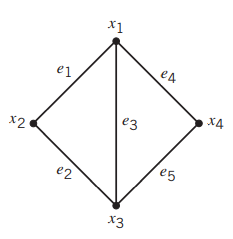
\includegraphics[width=4cm]{ex6.png}
    \captionsetup{labelformat=empty}
    \caption{\((G)\)}   
  \end{figure}
  

- Gọi \(N\) là tập hợp tất cả các cách tô \(n\) màu cho tất cả các đỉnh cho đồ thị \(G\). \\
- Ta có:

\[
    \begin{cases}
       \text{G có 4 đỉnh} & (1)\\
       \text{Mỗi đỉnh có } n \text{ cách.} & (2)
    \end{cases}
    \]
- Từ (1) và (2), theo nguyên lý nhân, ta suy ra được: \(N = n^{4}\) (\(n\) cách chọn cho mỗi đỉnh). \\
- Để tránh trường hợp các đỉnh kề nhau được tô cùng một màu:

\begin{itemize}
    \item Cho mỗi cạnh \(e_{i}\), gọi \(A_{i}\) là tập hợp tất cả các cách tô màu sao cho 2 đỉnh của cạnh \(e_{i}\) có cùng màu.
    \item Khi đó, \(N(\overline{A_{1}}\overline{A_{2}}\overline{A_{3}}\overline{A_{4}}\overline{A_{5}})\) là số cách tô \(n\) màu cần tìm.
\end{itemize}

- Theo nguyên lý bù trừ:
\begin{equation*}
    (\overline{A_{1}}\overline{A_{2}}\overline{A_{3}}\overline{A_{4}}\overline{A_{5}}) = |N| - S_{1} + S_{2} - S_{3} + S_{4} - S_{5}
\end{equation*}

\subparagraph{Tính \(S_{1}\)}\mbox{}\\

- Với mỗi cạnh \(e_{i}\), ta có:

\begin{itemize}
    \item Có \(n\) cách tô \(n\) màu cho hai đỉnh của cạnh \(e_{i}\)
    \item Có \(n^{2}\) cách tô \(n\) màu cho hai đỉnh còn lại.
\end{itemize}

\(\Rightarrow S_{1} = 5n^{3}\) (có tổng cộng 5 cạnh) 

\subparagraph{Tính \(S_{2}\)}\mbox{}\\

- Với mỗi hai cạnh \(e_{i}\) và \(e_{j}\), ta có:
\begin{itemize}
    \item Có \(n\) cách tô màu cho 3 đỉnh được nối bởi hai cạnh \(e_{i}\) và \(e_{j}\).
    \item Có \(n\) cách tô màu cho đỉnh còn lại.
\end{itemize}

\(\Rightarrow S_{2} =  \begin{pmatrix} 5 \\ 2 \\ \end{pmatrix}n^{2}\) (chọn 2 cạnh trong 5 cạnh) 


\subparagraph{Tính \(S_{3}\)}\mbox{}\\

- Với \(S_{3} = |A_{i}A_{j}{A_{k}}|\)
\begin{itemize}
    \item Với \((i,j,k) = (1,2,3)\), có \(n^{2}\) cách tô màu.
    \item Với \((i,j,k) = (3,4,5)\), có \(n^{2}\) cách tô màu.
    \item Với \((i,j,k) != (1,2,3) != (3,4,5)\), có \(n\) cách tô màu.
\end{itemize}

\(\Rightarrow S_{2} = 2n^{2}\left[\begin{pmatrix} 5 \\ 3 \\ \end{pmatrix} - 2\right] = 2n^{2} + 8n\)


\subparagraph{Tính \(S_{4}\) và \(S_{5}\)}\mbox{}\\

- Với 4 hay 5 cạnh, ta có:
\begin{itemize}
    \item Có \(n\) cách tô màu cho 4 đỉnh được nối bởi 4 hoặc 5 cạnh.
\end{itemize}

\(\Rightarrow S_{2} =  \begin{pmatrix} 5 \\ 4 \\ \end{pmatrix}n\) (chọn 4 cạnh trong 5 cạnh) \\

- Theo nguyên lý bù trừ:
\begin{align*}
    (\overline{A_{1}}\overline{A_{2}}\overline{A_{3}}\overline{A_{4}}\overline{A_{5}}) & = |N| - S_{1} + S_{2} - S_{3} + S_{4} - S_{5} \\
    & = n^{4} - 5n^{3} + \begin{pmatrix} 5 \\ 2 \\ \end{pmatrix}n^{2} - (2n^{2} + 8n) + \begin{pmatrix} 5 \\ 4 \\ \end{pmatrix}n-n \\
    & = n^{4} - 5n^{3} + 10n^{2} - (2n^{2} + 8n) + 5n -n \\
    & = n^{4} - 5n^{3} + 8n^{2} - 4n
\end{align*}

\section{Bài 7}
\begin{tcolorbox}
    \textbf{Đề bài:} Chứng minh rằng số cây khung của đồ thị đầy đủ \(K_{n}\) là \(n^{n-2}\).
    (với \(n > 1\)).
\end{tcolorbox}

- Theo định nghĩa của chuỗi Prufer:

\begin{center}
``Một cây \(n\) đỉnh được gán nhãn, có chuỗi Prüfer là một chuỗi với mỗi phần tử là nhãn từ  nhãn của cây, sao cho nó là chuỗi duy nhất để biểu diễn cây.''
\end{center}

- Ta cần chứng minh độ dài của chuỗi Prüfer là \(n-2\). \\
- Vậy chuỗi Prüfer cho ta một song ánh giữa hai tập hợp sau:

\begin{itemize}
    \item Tập hợp các cây \(n\) đỉnh được gắn nhãn                      (1)
    \item Tập hợp các chuỗi độ dài \(n-2\) với các số từ 1 đến \(n\)    (2)
\end{itemize}

- Trong đó tập hợp (1) chính là tập hợp các cây khung của một đồ thị đầy đủ \(n\) đỉnh. \\
- Và tập hợp (2) có lực lượng là \(n^{2}\) (với mỗi phần tử của chuỗi ta chọn được \(n\) số). \\
\(\Rightarrow\) Theo tính chất của song ánh, ta chứng minh được số cây khung của một đồ thị đầy đủ \(K_{n}\) là \(n^{n-2}\).

\section{Bài 8: Bài toán đường đi tránh vũng nước}
\begin{tcolorbox}
    \textbf{Đề bài:} Tìm thuật toán để giải quyết bài toán sau đây: Xét góc phần tư thứ I của hệ trục tọa độ \(Oxy\) với các lưới nguyên (giống như giấy tập có ô), có một vũng nước S ( là một tập hợp các điểm nguyên nằm trong I).
    (với \(n > 1\)).
\end{tcolorbox}

\begin{center}
    {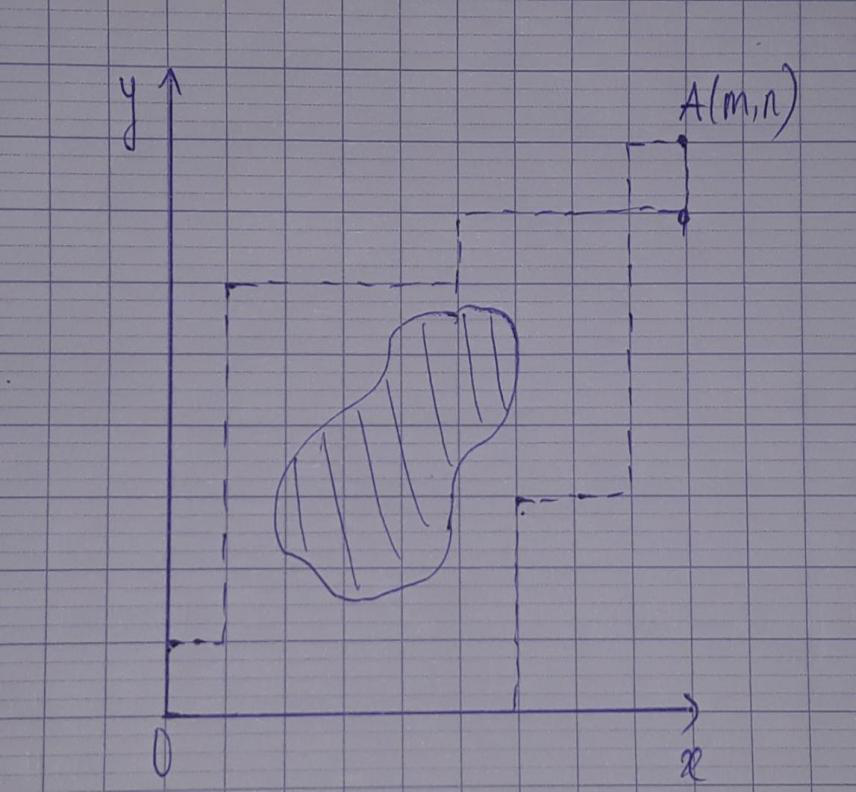
\includegraphics[width=8cm]{7.png}}
\end{center}

\subsection{Câu A}
\begin{tcolorbox}
    \textbf{Đề bài:} Tìm số đường đi từ O đến A tránh vũng nước S biết mỗi lần đi, chỉ được lên trên 1 đơn vị hoặc qua phải 1 đơn vị.
\end{tcolorbox}

\begin{itemize}
    \item Bắt đầu tại ô \(0,0\). Lần lượt đi từ trái qua phải, từ dưới lên trên và cập nhật giá trị cho các ô đã đi qua theo công thức đệ quy:
    \[ F(i,j) = 
    \begin{cases}
        1     & , (i,j) = (0,0) \\
        0     &, ij < 0 \\
        F(i + 1,j) + F(i, j + 1) 
    \end{cases}
    \]
    \item Lặp lại đến khi gán xong giá trị cho ô \(n,m\).
    \item Kết quả số đường đi từ \(O\) tới \(A\) là giá trị tại ô \(n,m\)
\end{itemize}

\subparagraph{Thuật toán}
\begin{verbatim}
    for(i =  0 -> m): F(i,n) = 1)
    for(j = 0 -> n - 1): F(m,j) = 1
    for(i = m - 1 -> 0; j = n - 1 -> 0):
        if(i,j) in S: F(i,j) = 0
        if (i,j) not in S: F(i,j) = F(i+1,j) + F(i,j+1)
\end{verbatim}

\(\Rightarrow F_{0,0}\)

\subsection{Câu B}
\begin{tcolorbox}
    \textbf{Đề bài:} Có nhận xét gì về số đường đi như vậy nếu vũng nước S không tồn tại.
\end{tcolorbox}

- Ta ký hiệu đường đi từ \(O\) đến \(A(m,n)\) với hai ký tự là \(L\) (lên trên) và \(P\)(qua phải). \\
- Dễ dàng nhận ra để di chuyển từ \(O\) đến \(A(m,n)\) luôn luôn cần \(m+n\) bước. \\
- Suy ra, số lượng ký tự \(P\) là \(m\) và số lượng ký tự \(L\) là \(n\). \\
- Dễ nhận thấy đổi chỗ các ký tự không làm thay đổi chuỗi. Vì vậy số đường đi của bài toán sẽ là số cách chọn \(m+n\) ký tự từ \(m\) ký tự \(P\) và \(n\) ký tự \(L\). Số cách chọn:

\begin{equation*}
    \begin{pmatrix} m + n \\ n \\ \end{pmatrix} = \begin{pmatrix} m + n \\ m \\ \end{pmatrix}
\end{equation*}
\section{Bài 9}
\begin{tcolorbox}
    \textbf{Đề bài:} Xét bài toán trên, tính số đường đi từ O đến A(n,n) và S là nửa mặt phẳng phía trên OA không kể bờ.
\end{tcolorbox}

- Tương tự, ta thấy đường đi từ \(O\) đến \(A(m,n)\) là một chuỗi có độ dài \(2n\) với hai ký tự là \(L\) (đi lên) và \(P\)(sang phải), trong đó số lượng mỗi ký tự là \(n\). \\
- Dễ thấy, số lượng ký tự P (sang phải) của ta luôn phải lớn hơn hoặc bằng số lượng ký tự \(L\) (đi lên). \\
- Vì nếu \(P < L\) thì ta sẽ chạm phải vũng nước. \\
- Từ đó, ta dễ dàng suy ra số lượng bước đi từ \(O\) đến \(A\) chính là số Catalan thứ \(n\):

\begin{equation*}
    C_{n} = \frac{1}{n+1}\begin{pmatrix} 2n \\ n \\ \end{pmatrix}
\end{equation*}

\section{Bài 10}
\begin{tcolorbox}
    \textbf{Đề bài:} Cho một hình chữ nhật \(mxn\). C là một bàn cờ nằm trong HCN này và \(C’\) là phần còn lại của \(C\) trong HCN đó.
    Chứng minh rằng \(R(x,C’)=x^{n} .R(1/x,C)\). Gợi ý: bt 15/351 quyển Applied Combinatorics.
\end{tcolorbox}

- Sử dụng định lý với \crule[cyan]{0.3cm}{0.3cm} là ô ở dòng n, cột m:
\begin{equation*}
    R_{n,m}(x) = xR_{n-1,m-1}(x) + R(E_{1},x)
\end{equation*}

- Trong đó, \(E_{1}\) là bàn cờ còn lại sau khi xóa \crule[cyan]{0.3cm}{0.3cm}. \\
- Tiếp tục sử dụng định lý với \crule[cyan]{0.3cm}{0.3cm} là ô ở dòng \(n\), cột \(m-1\): 

\begin{align*}
    R_{E_{1},x}(x) & = xR_{n-1,m-1}(x) + R(E_{2},x) \\
    \Rightarrow R_{n,m}(x) & = 2xR_{n-1,m-1}(x) + R(E_{2},x) 
\end{align*}

- Trong đó, \(E_{2}\) là bàn cờ còn lại sau khi xóa \crule[cyan]{0.3cm}{0.3cm}. \\
- Tiếp tục sử dụng định lý với \crule[cyan]{0.3cm}{0.3cm} là các ô còn lại của dòng \(n\), ta được:

\begin{equation*}
    R_{n,m}(x) = mxR_{n-1,m-1}(x) + R_{n-1,m}(x)
\end{equation*}

- Tìm đa thức quân xe của bàn cờ \(n\) dòng , \(m\) cột:

\[
    \begin{cases}
        r_{0}(n,m) = 1
        r_{1}(n,m) = nm
    \end{cases}
    \]

- Với 2 quân xe ta có \( \begin{pmatrix} n \\ 2 \\ \end{pmatrix} \) cách chọn vị trí dòng đặt quân xe. Với mỗi cách chọn dòng:

\begin{itemize}
    \item Quân xe thứ nhất có \(m\) cách chọn.
    \item Quân xe thứ hai có \(m-1\) cách chọn.
\end{itemize}

- Như vậy,

\begin{align*}
    r_{2}(n,m)  & = \begin{pmatrix} n \\ 2 \\ \end{pmatrix} \times  m \times (m-1) \\
                & = \begin{pmatrix} n \\ 2 \\ \end{pmatrix} \times  \frac{m!}{(m-3)!}
\end{align*}

- Lý luận tương tự, ta có:

\begin{equation*}
    r_{3}(n,m) = \begin{pmatrix} n \\ 3 \\ \end{pmatrix} \times \frac{m!}{(m-3)!}
\end{equation*}

- Tổng quát, ta được:

\begin{equation*}
    r_{k}(n,m) = \begin{pmatrix} n \\ k \\ \end{pmatrix} \times \frac{m!}{(m-k)!}
\end{equation*}

- Từ đó:

%\begin{equation*}
%    R_{n,m}(x) = \sum_{k = 0}^{n}  \begin{pmatrix} n \\ k \\ \end{pmatrix}\frac{(m)!}{(m-k)!}x^{k} (*) \\
%    \Rightarrow \frac{dR_{n,m}(x)}{dx} = \sum_{k = 1}^{n}  \begin{pmatrix} n \\ k \\ \end{pmatrix}\frac{(m)!}{(m-k)!}x^{k-1}

%\end{equation*}

\begin{align*}
    R_{n,m}(x) & = \sum_{k = 0}^{n} \begin{pmatrix} n \\ k \\ \end{pmatrix}\frac{(m)!}{(m-k)!}x^{k} \\
    \Rightarrow \frac{dR_{n,m}(x)}{dx} & = \sum_{k = 1}^{n} \begin{pmatrix} n \\ k \\ \end{pmatrix}\frac{(m)!}{(m-k)!}x^{k-1}
\end{align*}

- Từ (*), ta được:

\begin{align*}
    R_{n-1,m-1}(x)  & = \sum_{k = 0}^{n-1} \begin{pmatrix} n - 1 \\ k \\ \end{pmatrix}\frac{(m - 1)!}{(m - 1 - k)!}x^{k} \\
                    & = \sum_{k = 1}^{n} \begin{pmatrix} n - 1 \\ k - 1 \\ \end{pmatrix}\frac{(m - 1)!}{(m-k)!}x^{k-1} \\
    \Leftrightarrow nmR_{n-1,m-1}(x) & = \sum_{k = 0}^{n - 1}n\begin{pmatrix} n - 1 \\ k - 1 \end{pmatrix}\frac{m \times (m-1)!}{(m-k)!}x^{k-1} \\
                    & = \sum_{k = 1}^{n}n\begin{pmatrix} n \\ k \end{pmatrix}\frac{m!}{(m-k)!}x^{k-1} \\
                    & = \frac{dR_{n,m}(x)}{dx}
\end{align*}

\section{Bài 11: Định lý thặng dư Trung Hoa}
\begin{tcolorbox}
    \textbf{Đề bài:} Trước khi tiến hành thi học kì, toàn bộ sinh viên đh khtn bắt buộc phải được lấy mẫu tầm soát covid. Để biết chính xác có bao nhiêu sinh viên tham gia, chúng ta làm như sau (nhanh hơn và chính xác hơn việc đếm rất nhiều).
    Đầu tiên cho sinh viên tập trung trong khuôn viên trường là hình vuông cạnh 100m, để đảm bảo an toàn nên các bạn sinh viên đứng cách đều nhau. Lấy một ô đơn vị làm mẫu có kích thước 20m x 20m, ta dự đoán được trong đó có khoảng từ 490 đến 500 sinh viên. Sau đó chúng ta sẽ cho tất cả sinh viên xếp thành các hàng 5,7 và 11. Trong mỗi lần xếp như vậy, số sinh viên dư ra lần lượt là 0,4 và 3. Hãy tính chính xác số lượng sinh viên. (bởi vì dù chỉ 1 người chưa được tầm soát cũng rất nguy hiểm)
\end{tcolorbox}

- Gọi \(x\) là số lượng sinh viên cần tìm \(x \in \mathbb{N}\) \\
- Ta có số sinh viên của ĐH Khoa Học Tự Nhiên trong khoảng như sau: \\

\begin{align*}
    \frac{100\times 100\times 490}{20\times 20} & \leq x \leq \frac{100\times 100\times 500}{20\times 20} \\
    12250                     & \leq x \leq 12500 \text{ (*)}
\end{align*}

- Ta có hệ phương trình đồng dư:
\[
    \begin{cases}
        x & \equiv 0 \text{ (mod 5)} \\             
        x & \equiv 4 \text{ (mod 7)} \\
        x & \equiv 3 \text{ (mod 11)}
    \end{cases}
    \]

- Áp dụng định lý thặng dư Trung Hoa:
\[
    \begin{cases}
        M & = 5 \times 7 \times 11 = 385 \\             
        M_{1} & = 7 \times 11 = 77 \\
        M_{2} & = 5 \times 11 = 55 \\
        M_{3} & = 5 \times 7 = 35 \\
    \end{cases}
    \]

- Ta có:

\begin{itemize}
    \item \(y_{1} = 77^{-1} \text{ (mod 5)} = 2^{-1} \text{ (mod 5)} = 3\)
    \item \(y_{2} = 55^{-1} \text{ (mod 7)} = 6^{-1} \text{ (mod 7)} = 6\)
    \item \(y_{3} = 35^{-1} \text{ (mod 11)} = 2^{-1} \text{ (mod 11)} = 6\)
\end{itemize}

- Khi đó:

\[
    \begin{cases}
        x & \equiv 0\times 77\times 3 + 4\times 55\times 6 + 3\times 35\times 6 \text{ (mod 385)} \\             
        x & \equiv 1950 \text{ (mod 385)} \\
        x & \equiv 25 \text{ (mod 385)}
    \end{cases}
    \]
- Suy ra \(x\) có dạng :

\begin{equation*}
    x = 25 + 385k, (k \in \mathbb{N})
\end{equation*}

- Kết hợp với \((*)\): 

\begin{align*}
    & 12250                     \leq 25 + 385k \leq 12500 \\
    & \Leftrightarrow 31,8                       \leq k \leq 32,4 \\
    & \Rightarrow k  = 32
\end{align*}

- Vậy số lượng sinh viên cần tìm là:
\begin{equation*}
    x = 375 + 385 \times 32 = 12345
\end{equation*}

\end{sloppypar}
\end{document}
